\section{TEST SECTION} \normalfont

\begin{dissQuote}{\~{}anon}
    This is just a test that you can write quotes. This is how it will look at the end. If you dislike, you can change in dissetation.cls
\end{dissQuote}
 
%Before you start any text in any section you must write the command \textit{\{\textbackslash fontfamilty\{ptm\}\textbackslash selectfont RND TEXT \}}.

Before you start any text in any section your must write the command \textbackslash{normalfont} so the text is in Times New Roman (the one that the word template has). 

%to cite you shouldn't use the typical \textit{\textbackslash{cite\{paper\_name\}}}, you need to use \textit{\textbackslash{citen\{paper\_name\}}} because we are using the multibib package to have the publication list of the included work and the typical references.

Since I know y'all want to use fancy formulas in your \LaTeX{} project, here you have a very simple one~\cref{eq:simple-eq}.

\begin{equation} \label{eq:simple-eq}
D_{NMP} = \min \left\{ \dfrac{\#MesoPat}{Max_{chambers}}, 1.0 \right\}
\end{equation}

And just in case you wanted something a bit more complex written but simple to calculate you have this Equation~\ref{eq:convoluted-eq}!.

\begin{equation} \label{eq:convoluted-eq}
spa(x)= \dfrac{\sum_{i=1}^{\left | clusts \right |}\sum_{j=1, j\neq i}^{\left | clusts \right |}\dfrac{Dist(clust_{i}, clust_{j})}{\left | room \right |}}{\left | clusts \right | \cdot (\left | clusts \right | - 1)}
\end{equation}

\subsection{Sub section} \normalfont

This is the example of how a subsection would look like! \cite{Kegel2020-surveyPuzzles}.

Multiple citations could look like this \cite{alvarez2020-designerpersonas,yannakakis2014micc}, and this is to refer to a figure! \cref{fig:myRNDFig} or the classic Figure~\ref{fig:myRNDFig}.

\begin{figure}[h]
    \centering
    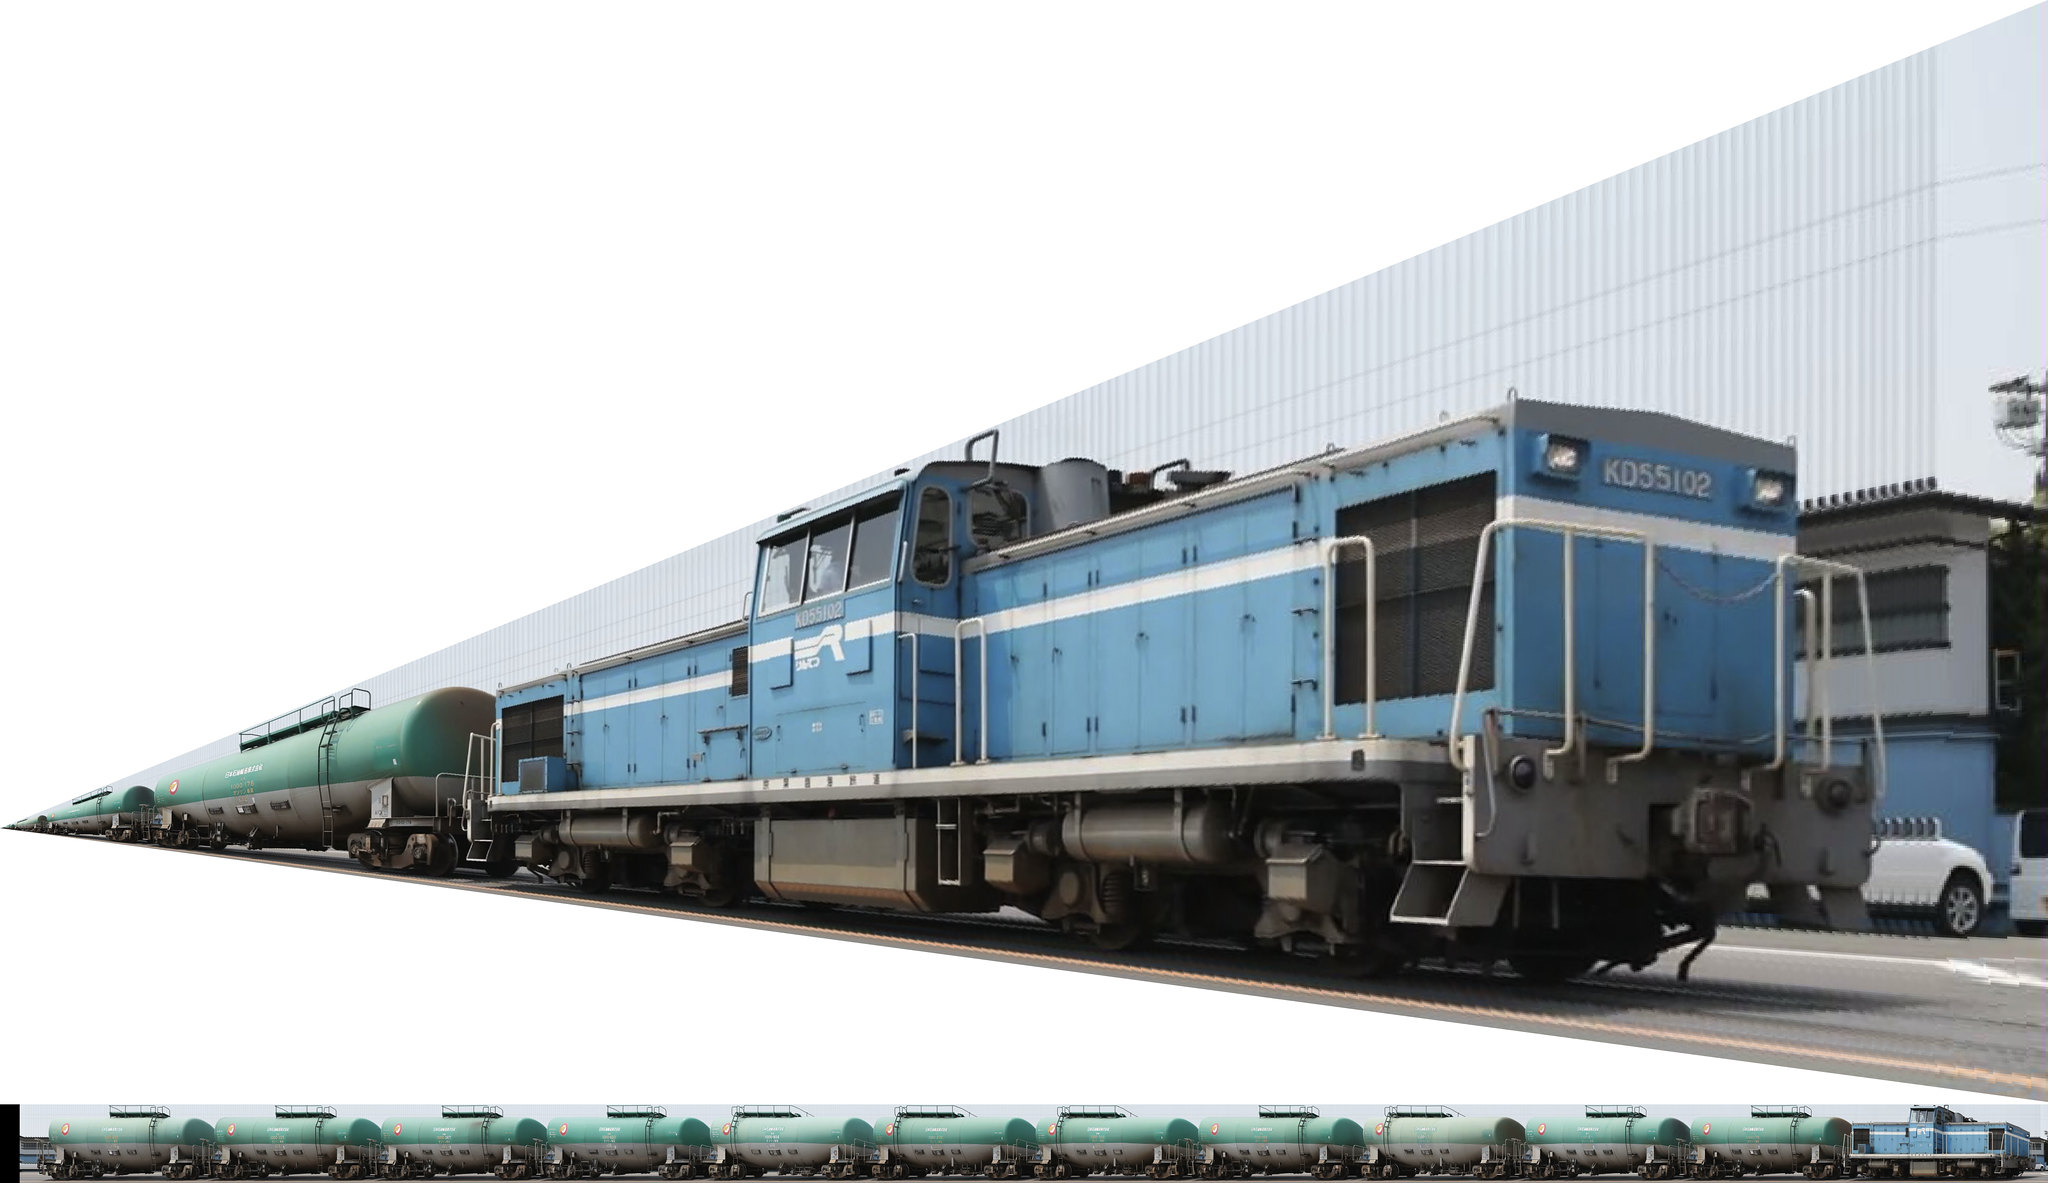
\includegraphics[width=\linewidth]{figures/example-1.jpg}
        \caption{This is a random figure added here}
    \label{fig:myRNDFig}
\end{figure}

Another thing that you might be interested in changing is the separation between paragraphs. There is a comment in the dissertation.cls with brief instructions on how to change that! Specifically, you are interested in changing this \textit{\textbackslash{setlength}\{\textbackslash{parskip}\}\{size\_em\}}. \textbf{OBS!} This might force you to change the many \textit{\textbackslash{vspace}\{value\}} that exists around all the class. 

\subsubsection{Deeper level}

This is the maximum level you should use, it is not too common to use deeper levels such as subsubsubsection as it can be observed in Table~\ref{table:sectionKnowledge} or~\cref{table:sectionKnowledge}.

\blindtext

\begin{table}
\begin{center}
\begin{tabular}{lccccc}
\hline
\rule{0pt}{12pt}
True Information&paper&$\Diamond$&$\Box$&$\bigtriangleup$ 
\\ 
\hline
\\[-6pt]
No & Paper 1 & 3 & 3 & 0 \\ 
Noup & Paper 2 & 3 & 3 & 0 \\ 
No & Paper 3 & 2 & 7 & 0 \\ 
Nah & Paper 4 & 5 & 3 & 0 \\ 
No & Paper 5 & 4 & 1 & 0 \\ 
Noup & Paper 6 & 5 & 0 & You wish \\ 
\hline
\\[-6pt]
\multicolumn{6}{l}{$\Diamond$ subsections\ \
$\Box$ subsubsections\ \
$\bigtriangleup$ subsubsubsections}
\end{tabular}
{\caption{Non-extensive and non-real table of papers that actually use different levels of sections. The information in this table could not be more fake so do not consider for your study :)\dots{} You can use this to create your tables if wanted: https://www.tablesgenerator.com/}\label{table:sectionKnowledge}}
\end{center}
\end{table}

However, if you really need subsubsubsections, then you can use the following:

\paragraph{This is a new subsubsubsection}
You define a subsubsubsection with the command \textit{\textbackslash paragraph} but normally you wouldn't need a subsubsubsection. 

\blindtext
\blindtext